\باب{گاؤس کا قانون اور پھیلاو}
\حصہ{ساکن چارج}

\حصہ{فیراڈے کا تجربہ}
اس باب کا آغاز جناب \ترچہ{مائکل فیراڈے}\حاشیہب{Michael Faraday} کے ایک تجربے سے کرتے ہیں جس کے نتیجے کو یوں بیان کیا جا سکتا ہے۔چارج \عددیء{Q} کو غیر چارج شدہ موصل سطح میں مکمل طور پر یوں بند کرنے کے بعد، کہ چارج اور سطح  کہیں بھی ایک دونوں کو نہ چھوئیں، موصل سطح کو زمین کے ساتھ ایک لمحے کے لئے ملانے سے موصل سطح پر \عددیء{-Q} چارج پیدا ہو جاتا ہے۔\حاشیہط{بہتری درکار ہے}دیکھا یہ گیا ہے کہ چارج اور بیرونی سطح کے درمیان فاصلہ کم یا زیادہ کرنے سے نتیجے پر کوئی اثر نہیں ہوتا۔اسی طرح چارج اور سطح کے درمیان مختلف غیر موصل مواد بھرنے سے بھی نتیجے پر کوئی اثر نہیں ہوتا۔مزید یہ کہ سطح کی شکل کا بھی نتیجے پر کوئی اثر نہیں ہوتا۔اسی طرح جس چیز پر چارج \عددیء{Q} رکھا گیا ہو، اس کی شکل کا بھی نتیجے پر کوئی اثر نہیں ہوتا۔ 

ایسا معلوم ہوتا ہے جیسے اندرونی چارج سے بیرونی سطح تک چارج کی مقدار اور قطب کی خبر پہنچتی ہے۔اس حقیقت کو تصوراتی جامع یوں پہنایا جا سکتا ہے کہ ہم سمجھیں کہ مثبت چارج سے ہر جانب یکساں طور پر کچھ خارج ہوتا ہے۔اس چیز کو ہم \اصطلاح{برقی بہاو}\فرہنگ{برقی بہاو}\حاشیہب{electric flux}\فرہنگ{electric flux}  کہیں گے اور اس کو \عددیء{\psi} سے ظاہر کریں گے۔برقی بہاو کو چارج کے برابر تصور کیا جاتا ہے۔
\begin{align}
\psi=Q
\end{align}
برقی بہاو کی اکائی  کولومب \عددیء{\si{\coulomb}} ہی تصور کی جاتی ہے۔منفی چارج کی صورت میں برقی بہاو کی سمت الٹی ہو گی اور یہ چارج میں داخل ہو گا۔

تصور کریں کہ اندرونی چارج  \عددیء{r_1} رداس کی کرہ پر پایا جاتا ہے جبکہ اسے  \عددیء{r_2} رداس کی کرہ نے گھیرا ہوا ہے۔کرہ کی سطح \عددیء{4\pi r^2} کے برابر ہوتی ہے۔اندرونی کرہ سے  \عددیء{\psi} برقی بہاو خارج ہوتا ہے۔یوں اندرونی کرہ سے \عددیء{\tfrac{\psi}{4\pi r_1^2}} برقی بہاو فی اکائی رقبہ خارج ہوتا ہے  جسے \عددیء{\tfrac{Q}{4\pi r_1^2}} لکھا جا سکتا ہے۔ اسی طرح بیرونی کرہ پر \عددیء{\tfrac{Q}{4\pi r_2^2}} برقی بہاو فی اکائی رقبہ پہنچتی ہے۔برقی بہاو فی اکائی رقبے کو \اصطلاح{برقی بہاو کی کثافت}\فرہنگ{کثافت!برقی بہاو}\حاشیہب{electric flux density}\فرہنگ{density!electric flux} \عددیء{D} کہا جائے گا۔یوں اگر اندرونی کرہ کے رداس کو اتنا کم کر دیا جائے کہ اس کو نقطہ تصور کرنا ممکن ہو اور اس نقطہ چارج کو رداس \عددیء{r} کے کرہ کے مرکز پر رکھا جائے تو کرہ پر
\begin{align}\label{مساوات_گاؤس_نقطہ_چارج_کے_بہاو_کی_کثافت}
\kvec{D}=\frac{Q}{4\pi r^2} \ar
\end{align}
سمتیہ برقی بہاو کی کثافت پائی جائے گی۔صفحہ \حوالہصفحہ{مساوات_کولومب_نقطہ_چارج_کروی_رداس_پر_تبدیل_نہیں_ہوتا} پر مساوات \حوالہ{مساوات_کولومب_نقطہ_چارج_کروی_رداس_پر_تبدیل_نہیں_ہوتا} سے موازنہ کرنے سے ثابت ہوتا ہے کہ خالی خلاء میں
\begin{align}\label{مساوات_گاؤس_میدان_اور_کثافت_کا_تعلق}
\kvec{D}=\epsilon_0 \kvec{E} \hspace{2cm} \textrm{خالی خلاء}
\end{align}
کے برابر ہے۔اگر نقطہ چارج کو کروی محدد کے مرکز پر نہ رکھا جائے تب کسی بھی مقام پر برقی بہاو کی کثافت حاصل کرنے کی خاطر مساوات \حوالہ{مساوات_گاؤس_نقطہ_چارج_کے_بہاو_کی_کثافت} یوں لکھی جائے گی
\begin{align}\label{مساوات_گاؤس_کسی_بھی_جگہ_نقطہ_چارج_کے_بہاو_کی_کثافت}
\kvec{D}=\frac{Q}{4\pi R^2} \kvec{a}_R
\end{align}
جہاں \عددیء{\kvec{a}_R} چارج  سے اس مقام کی جانب اکائی سمتیہ ہے اور \عددیء{R} ان کے درمیان فاصلہ ہے۔

کسی بھی حجم جس میں تغیر پذیر  چارج کی کثافت پائی جائے میں مقام \سمتیہ{r'} پر \عددیء{\Delta h'} حجم میں \عددیء{\rho_h' \Delta h'}  چارج پایا جائے گا جو مقام \سمتیہ{r} پر
\begin{align*}
\Delta \kvec{D}(\kvec{r})=\frac{\rho_h' \Delta h'}{4\pi \abs{\kvec{r}-\kvec{r'}}^2} \frac{\kvec{r}-\kvec{r'}}{\abs{\kvec{r}-\kvec{r'}}}
\end{align*} 
برقی بہاو کی کثافت پیدا کرے گا۔حجم کے تمام چارجوں سے
\begin{align}\label{مساوات_گاؤس_حجم_چارج_کے_بہاو_کی_کثافت}
\kvec{D}(\kvec{r})=\int\limits_{h}\frac{\rho_h' \dif h'}{4\pi \abs{\kvec{r}-\kvec{r'}}^2} \frac{\kvec{r}-\kvec{r'}}{\abs{\kvec{r}-\kvec{r'}}}
\end{align} 
حاصل ہو گا۔مساوات \حوالہ{مساوات_گاؤس_حجم_چارج_کے_بہاو_کی_کثافت} کا صفحہ \حوالہصفحہ{مساوات_کولومب_حجم_چارج_کا_میدان} پر مساوات \حوالہ{مساوات_کولومب_حجم_چارج_کا_میدان} کے ساتھ موازنہ کرنے سے ثابت ہوتا ہے کہ حجمی کثافت کے لئے بھی مساوات \حوالہ{مساوات_گاؤس_میدان_اور_کثافت_کا_تعلق} خالی خلاء میں \سمتیہ{D} اور \سمتیہ{E} کا تعلق بیان کرتا ہے۔اسی طرح \عددیء{\rho_S} اور \عددیء{\rho_L} سے پیدا \عددیء{\kvec{D}} اور \عددیء{\kvec{E}} کا خالی خلاء میں تعلق بھی مساوات \حوالہ{مساوات_گاؤس_میدان_اور_کثافت_کا_تعلق}  ہی بیان کرتا ہے۔یوں  مساوات \حوالہ{مساوات_گاؤس_میدان_اور_کثافت_کا_تعلق} ایک عمومی مساوات ہے۔

\حصہ{گاؤس کا قانون}
فیراڈے کے تجربے کو قانون کی شکل میں یوں پیش کیا جا سکتا ہے جسے \اصطلاح{گاؤس کا قانون}\فرہنگ{گاؤس کا قانون}\حاشیہب{Gauss's law}\فرہنگ{Gauss's law} کہتے ہیں۔

\ابتدا{قانون}
کسی بھی مکمل بند سطح سے  کل گزرتی برقی بہاو سطح میں گھیرے چارج کے برابر ہوتی ہے۔
\انتہا{قانون}
جناب گاؤس\حاشیہب{Carl Friedrich Gauss} نے اس قانون کو ریاضیاتی شکل دی جس کی بنا پر یہ قانون انہیں کے نام سے منسوب ہے۔آئیں گاؤس کے قانون کی ریاضیاتی شکل حاصل کریں۔
\begin{figure}
\centering
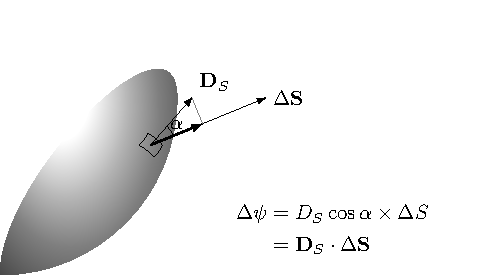
\includegraphics{figGaussBalloon}
\caption{مکمل بند سطح سے گزرتی برقی بہاو سطح میں گھیرے کل چارج کے برابر ہے۔}
\label{شکل_گاؤس_کا_قانون}
\end{figure}

شکل \حوالہ{شکل_گاؤس_کا_قانون} میں  بند سطح دکھائی گئی ہے جس کی کوئی مخصوص شکل نہیں ہے۔اس سطح کے اندر یعنی سطح کے گھیرے حجم میں کل \عددیء{Q} چارج  پایا جاتا ہے۔سطح پر کسی بھی مقام سے گزرتا برقی بہاو اس مقام پر سطح کی عمودی سمت میں برقی بہاو کی کثافت اور اس مقام کے رقبہ کے حاصل ضرب کے برابر ہو گا۔یوں شکل کو دیکھتے ہوئے  چھوٹے سے رقبہ \عددیء{\Delta S} پر سطح کے عمودی سمت میں برقی بہاو کے کثافت  کی قیمت \عددیء{D_S \cos \alpha} ہو گی لہٰذا
\begin{align*}
\Delta \psi =D_S \cos \alpha  \Delta S
\end{align*}
ہو گا۔کثافتِ برقی بہاو \عددیء{D_S} لکھتے ہوئے زیرنوشت میں \عددیء{S} اس حقیقت کی یاد دہانی کراتا ہے کہ سطح پر کثافتِ برقی بہاو کی قیمت کی بات کی جا رہی ہے۔اس مساوات کو ضرب نقطہ کے استعمال سے
\begin{align*}
\Delta \psi =\kvec{D}_S \cdot \Delta \kvec{S}
\end{align*}
لکھا جا سکتا ہے۔مکمل سطح سے گزرتے کل برقی بہاو تکملہ سے حاصل ہو گی جو گاؤس کے قانون کے مطابق گھیرے ہوئے چارج \عددیء{Q} کے برابر ہے۔یوں
\begin{align}
\psi=\oint\limits_{S} \kvec{D}_S \cdot \Delta \kvec{S}=Q
\end{align}
لکھا جا سکتا ہے۔یہ تکملہ دراصل دو درجی  تکملہ ہے جسے ہم عموماً ایک درجی تکملہ سے ہی ظاہر کریں گے۔تکملہ کے نشان پر گول دائرہ بند تکملہ\فرہنگ{بند تکملہ}\حاشیہب{closed integral} کو ظاہر کرتا ہے جبکہ بند تکملہ  کے  نیچے \عددیء{S} اس بند سطح کو ظاہر کرتا ہے جس پر بند تکملہ حاصل کیا جا رہا ہو۔اس بند سطح کو عموماً \اصطلاح{گاؤس سطح}\فرہنگ{گاؤس سطح}\حاشیہب{gaussian surface}\فرہنگ{gaussian surface} کہتے ہیں۔

جس مقام پر چارج کی کثافت \عددیء{\rho_h} ہو، وہاں  چھوٹی سی حجم \عددیء{\Delta h} میں کل چارج \عددیء{\rho_h \Delta h}  پایا جاتا ہے۔یوں کسی بھی حجم کو چھوٹے چھوٹے حصوں میں تقسیم کرتے ہوئے تمام حصوں میں پائے جانے والے چارجوں کا مجموعہ پوری حجم میں چارج کے برابر ہو گا یعنی
\begin{align}\label{مساوات_گاؤس_کل_حجمی_چارج}
Q=\int\limits_{h} \rho_h \dif h
 \end{align}
جہاں تین درجی حجم کے تکملہ کو ایک درجی تکملہ کے نشان سے ظاہر کیا گیا ہے۔

مندرجہ بالا دو مساوات سے
\begin{align}\label{مساوات_گاؤس_کے_قانون_کی_تکملہ_شکل}
\oint\limits_{S} \kvec{D}_S \cdot \Delta \kvec{S}=\int\limits_{h} \rho_h \dif h
\end{align}
حاصل ہوتا ہے جو گاؤس کے قانون کی تکملہ شکل ہے۔اس مساوات کو یوں پڑھا جاتا ہے کہ کسی بھی بند سطح سے گزرتی کل برقی بہاو اس سطح کے اندر گھیرے کل چارج کے برابر  ہے۔

یہ ضروری نہیں کہ گھیرے ہوئے حجم یعنی بند حجم میں حجمی کثافت ہی پائی جائے۔بند حجم کے اندر  سطحی کثافت، لکیری کثافت، علیحدہ علیحدہ نقطہ چارج یا ان تینوں اقسام کا مجموعہ پایا جا سکتا ہے۔حجم گھیرنے والے بند بیرونی سطح کے اندر کسی سطح پر  سطحی کثافت کی صورت میں مساوات \حوالہ{مساوات_گاؤس_کل_حجمی_چارج} کی جگہ
\begin{align}
Q&=\int\limits_{S} \rho_S \dif S
\end{align}
لکھا جائے گا جہاں چارج بردار سطح ازخود بند یا کھلی سطح ہو سکتی ہے۔لکیری کثافت کی صورت میں
\begin{align}
Q&=\int\limits_{L} \rho_L \dif L
\end{align}
جبکہ  \عددیء{n} عدد نقطہ چارج کی صورت میں
\begin{align}
Q=\sum_n Q= Q_1+Q_2+\cdots
\end{align}
لکھا جائے گا، وغیرہ وغیرہ۔بہرحال مساوات \حوالہ{مساوات_گاؤس_کل_حجمی_چارج} سے مراد یہ تمام صورتیں لی جاتی ہیں اور یوں ان تمام صورتوں کے لئے گاؤس کے  قانون کی تکملہ شکل مساوات \حوالہ{مساوات_گاؤس_کے_قانون_کی_تکملہ_شکل} ہی ہے۔


%=============
\حصہ{گاؤس کے قانون کا استعمال}
گزشتہ باب میں ہم نے کولومب کے قانون سے نقطہ چارج، لامحدود  لکیری چارج اور لامحدود سطحی چارج  سے پیدا برقی میدان حاصل کئے۔آئیں انہیں کو  گاؤس کے قانون کی مدد سے بھی حاصل کریں۔ آپ دیکھیں گے کہ ان تینوں صورتوں میں گاؤس کے قانون کا استعمال شرم ناک حد تک سادہ ثابت ہو گا۔یہاں یہ بتلانا ضروری ہے کہ ایسے  مسائل جن میں گاؤس کا قانون استعمال کیا جا سکے کی تعداد  بہت کم ہیں۔

\جزوحصہ{نقطہ چارج}
شکل \حوالہ{شکل_گاؤس_کرہ_کی_سطح_پر_مرکز_کے_نقطہ_چرج_کا_میدان} میں کرہ کے مرکز پر نقطہ چارج دکھایا گیا ہے۔ نقطہ چارج کو کروی محدد\حاشیہب{spherical coordinates} کے مرکز پر رکھتے ہوئے ہم  نے مختلف مقامات سے دیکھتے ہوئے مسئلے کی مشابہت کی بنا پر اخذ کیا تھا کہ کثافتِ برقی میدان صرف رداس کی سمت میں ممکن ہے اور اس  کی حتمی قیمت صرف اور صرف رداس \عددیء{r} تبدیل کرنے سے تبدیل ہو گی۔اس کا مطلب ہے کہ کروی محدد کے مرکز کے گرد رداس \عددیء{r} کے کرہ  پر \سمتیہ{D} تبدیل نہیں ہو گا۔
\begin{figure}
\centering
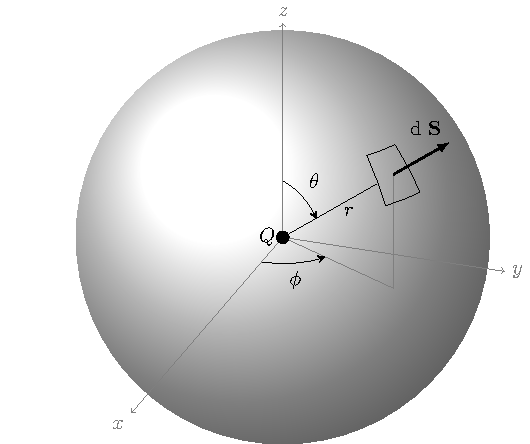
\includegraphics{figGaussSphere}
\caption{کرہ کے مرکز پر نقطہ چارج کا کرہ کے سطح پر کثافتِ برقی بہاو}
\label{شکل_گاؤس_کرہ_کی_سطح_پر_مرکز_کے_نقطہ_چرج_کا_میدان}
\end{figure}

کروی محدد استعمال کرتے ہوئے کرہ پر چھوٹی سی سطح
\begin{align*}
\dif S=r^2 \sin \theta \dif \theta \dif \phi
\end{align*}
لکھی جا سکتی ہے۔اسی کی سمتی شکل
\begin{align*}
\dif \kvec{S}=r^2 \sin \theta \dif \theta \dif \phi \ar
\end{align*}
ہو گی۔اس سطح پر کثافتِ برقی بہاو کی قیمت \عددیء{D_S} اور سمت \عددیء{\ar} ہو گی لہٰذا سمتی کثافتِ برقی بہاو 
\begin{align*}
\kvec{D}_S=D_S \ar
\end{align*}
لکھی جائے گی۔یوں اس چھوٹی سی سطح سے گزرتی برقی بہاو
\begin{align*}
\dif \psi&=\kvec{D}_S \cdot \dif \kvec{S}\\
&=\left( D_S \ar \right) \cdot \left(r^2 \sin \theta \dif \theta \dif \phi \ar \right)\\
&= D_S r^2 \sin \theta \dif \theta \dif \phi
\end{align*}
ہو  گی۔اس طرح پوری کرہ سے گزرتی برقی بہاو تکملہ سے یوں حاصل ہو گی۔
\begin{align*}
\psi&=D_S r^2  \int_{\phi=0}^{\phi=2\pi}\int_{\theta=0}^{\theta=\pi} \sin \theta \dif \theta \dif \phi\\
&=D_S r^2 \int_{\phi=0}^{\phi=2\pi} \eval{-\cos \theta}_0^{\pi} \dif \phi\\
&=D_S r^2 \int_{\phi=0}^{\phi=2\pi} 2 \dif \phi\\
&=4 \pi r^2 D_S
\end{align*}
گاؤس کے قانون کے تحت یہ برقی بہاو گھیرے گئے چارج \عددیء{Q} کے برابر ہے لہٰذا
\begin{align*}
4 \pi r^2 D_S=Q
\end{align*}
ہو گا جس سے
\begin{align*}
D_S=\frac{Q}{4 \pi r^2}
\end{align*}
حاصل ہوتا ہے۔یہی جواب بغیر زیادہ حساب و کتاب کے یوں حاصل کیا جا سکتا ہے۔

کرہ پر کثافتِ برقی بہاو \عددیء{D_S} عمودی ہے اور اس کی قیمت کرہ پر تبدیل نہیں ہوتی۔کرہ کی سطح \عددیء{4\pi r^2} کے برابر ہے لہٰذا پوری سطح سے \عددیء{4\pi r^2 D_S} برقی بہاو گزرے گی جو گاؤس کے قانون کے تحت \عددیء{Q} کے برابر ہے لہٰذا \عددیء{4\pi r^2 D_S=Q} ہو گا جس سے \عددیء{D_S=\tfrac{Q}{4\pi r^2}} حاصل ہوتا ہے۔اس کی سمتی شکل
\begin{align}
\kvec{D}_S=\frac{Q}{4\pi r^2} \ar
\end{align}
اور \عددیء{\kvec{D}=\epsilon_0 \kvec{E}} سے
\begin{align}
\kvec{E}=\frac{Q}{4\pi \epsilon_0 r^2} \ar
\end{align}
حاصل ہوتا ہے۔اس مساوات کا صفحہ \حوالہصفحہ{مساوات_کولومب_نقطہ_چارج_کروی_رداس_پر_تبدیل_نہیں_ہوتا} پر مساوات \حوالہ{مساوات_کولومب_نقطہ_چارج_کروی_رداس_پر_تبدیل_نہیں_ہوتا} کے ساتھ موازنہ کریں اور دیکھیں کہ موجودہ جواب کتنی آسانی سے حاصل ہوا۔

\جزوحصہ{یکساں چارج بردار سیدھی لامحدود لکیر}
ایسی لامحدود لکیر جس پر چارج کی یکساں کثافت پائی جائے کے گرد رداس پر گھومتے ہوئے  صورت حال میں کوئی تبدیلی نظر نہیں آتی۔اسی طرح اس لکیر کے ساتھ ساتھ چلتے ہوئے بھی صورت حال میں کسی قسم کی تبدیلی پیدا نہیں ہوتی۔لامحدود لکیر کو نلکی محدد کی \عددیء{z} محدد تصور کرتے  ہوئے  ان حقائق کی روشنی میں ہم توقع کرتے ہیں کہ برقی میدان صرف  رداس تبدیل کرنے سے ہی تبدیل ہو گا۔مزید، جیسا کہ پچھلی باب میں بتلایا گیا، کسی بھی نقطے کے ایک جانب لکیر پر چارج سے پیدا برقی میدان کا وہ حصہ جو \عددیء{\az} کی سمت میں ہو کو لکیر پر نقطے کی دوسری جانب برابر فاصلے  پر چارج سے پیدا برقی میدان کا وہ حصہ جو \عددیء{\az} کی سمت میں ہو  ختم کرتا ہے۔یوں یہ اخذ کیا جا سکتا ہے کہ کثافتِ برقی بہاو صرف رداس کی سمت میں ہی پایا جائے گا۔آئیں ان معلومات کی روشنی میں گاؤس کے قانون کی مدد سے کثافتِ برقی بہاو حاصل کریں۔

چارج بردار لکیر جس پر یکساں کثافتِ چارج \عددیء{\rho_L} پایا جائے  کی لمبائی \عددیء{L} میں کل چارج \عددیء{\rho_L L} ہو گا۔اس لمبائی کے گرد \عددیء{\rho} رداس کی نلکی سطح تصور کرتے ہیں جس کے دونوں آخری سرے\حاشیہد{آخری سروں کو غیر موصل چادر سے بند کیا جا سکتا ہے۔یوں اس نلکی سطح تک چارج نہیں پہنچ پائے گا۔} بند تصور کریں۔چونکہ برقی بہاو صرف رداس کی سمت میں ہے لہٰذا ان دونوں آخری سروں سے کوئی برقی بہاو نہیں ہو گا۔نلکی سطح کا رقبہ \عددیء{2\pi \rho L} ہے جبکہ اس سطح پر ہر جگہ کثافتِ برقی بہاو  \عددیء{D_{\rho}} ہے لہٰذا پوری سطح سے \عددیء{2\pi \rho L D_{\rho}} برقی بہاو ہو گا جو گاؤس کے قانون کے تحت گھیرے گئے چارج \عددیء{\rho_L L} کے برابر ہو گا۔اس طرح
\begin{align*}
2 \pi \rho D_{\rho} = \rho_L L
\end{align*}
لکھتے ہوئے
\begin{align*}
D_{\rho}=\frac{\rho_L}{2\pi \rho}
\end{align*}
حاصل ہوتا ہے جس کی سمتی شکل
\begin{align}\label{مساوات_گاؤس_لکیری_کثافت_کا_میدان}
\kvec{D}_S=\frac{\rho_L}{2\pi \rho} \arho
\end{align}
سے 
\begin{align*}
\kvec{E}_S=\frac{\rho_L}{2\pi \epsilon_0\rho} \arho
\end{align*}
حاصل ہوتا ہے۔صفحہ \حوالہصفحہ{مساوات_کولومب_لامحدود_لکیر_رداسی_میدان_پیدا_کرتا_ہے} پر مساوات \حوالہ{مساوات_کولومب_لامحدود_لکیر_رداسی_میدان_پیدا_کرتا_ہے} کے ساتھ موازنہ کریں اور دیکھیں کہ موجودہ طریقہ کتنا سادہ ہے۔
%=============
\حصہ{ہم محوری تار}
یکساں چارج بردار سیدھی لامحدود لکیر کے قصے کو آگے بڑھاتے ہوئے تصور کریں کہ اس تار کا رداس \عددیء{\rho_1} ہے۔اگر تار پر کسی بھی  جگہ \عددیء{L} لمبائی میں \عددیء{Q} چارج پایا جائے تو تار پر چارج کی لکیری کثافت  \عددیء{\rho_L=\tfrac{Q}{L}} ہو گی جبکہ اس پر چارج کی سطحی کثافت \عددیء{\tfrac{Q}{2\pi \rho_1 L}} ہو گی۔جیسا آپ جانتے ہیں ہیں ٹھوس موصل میں چارجوں کے مابین قوت دفع کی وجہ سے تمام  چارج موصل کے بیرونی سطح پر دکھیلے جاتے ہیں۔یوں چارج \عددیء{Q} تار  کے  بیرونی سطح محور سے \عددیء{r_1} فاصلے پر پایا جائے گا۔

\begin{figure}
\centering
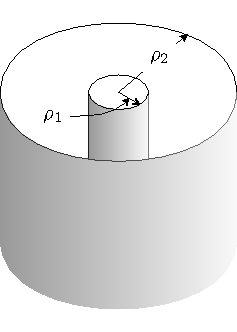
\includegraphics{figGaussCoaxial}
\caption{ہم محوری تار}
\label{شکل_گاؤس_ہم_محوری_تار}
\end{figure}

اب تصور کریں کہ پہلی تار کے اوپر نلکی نما دوسری تار چڑھائی جائے جس کا اندرونی رداس \عددیء{\rho_2} ہو جہاں \عددیء{\rho_2 > \rho_1} ہو گا۔ایسی تار جسے \اصطلاح{ہم محوری تار}\فرہنگ{ہم محوری تار}\حاشیہب{coaxial cable}\فرہنگ{coaxial cable} کہتے ہیں کو شکل \حوالہ{شکل_گاؤس_ہم_محوری_تار} میں دکھایا گیا ہے۔تصور کریں کہ بیرونی تار پر کسی بھی جگہ \عددیء{L} لمبائی پر \عددیء{-Q} چارج پایا جاتا ہے۔دونوں تاروں پر الٹ اقسام کے چارج ہیں جن میں قوت کشش پائی جائے گی۔یوں بیرونی تار پر چارج تار کے اندرونی سطہ یعنی محور سے \عددیء{\rho_2} رداس پر پایا جائے گا۔بیرونی تار پر \عددیء{\rho_L=\tfrac{-Q}{L}} جبکہ \عددیء{\rho_S=\tfrac{-Q}{2\pi \rho_2 L}} ہو گی۔

دونوں تاروں کے درمیانی فاصلے میں رداس \عددیء{\rho} کی فرضی نلکی سطح صرف اندرونی تار کے چارج کو گھیرتی ہے لہٰذا \عددیء{L} لمبائی کی ایسی نلکی  پر مساوات \حوالہ{مساوات_گاؤس_لکیری_کثافت_کا_میدان} کی طرح
\begin{align}
\kvec{D}&=\frac{\rho_L}{2\pi \rho} \arho\\
&=\frac{Q}{2\pi \rho L} \arho
\end{align}  
پایا جائے گا۔آپ دیکھ سکتے ہیں کہ بیرونی تار  پر چارج  کا اس میدان پر کوئی اثر نہیں پایا جاتا۔یوں اندرونی تار کی سطح پر
\begin{align}
\kvec{D}_1=\frac{Q}{2\pi \rho_1 L} \arho
\end{align}
جبکہ بیرونی تار کے اندرونی سطح پر
\begin{align}
\kvec{D}_2=\frac{Q}{2\pi \rho_2 L} \arho
\end{align}
پایا جائے گا۔بیرونی تار کے باہر فرضی نلکی سطح میں کل صفر چارج پایا جاتا ہے لہٰذا ہم محوری تار کے باہر
\begin{align}\label{مساوات_گاؤس_ہم_محوری_تار_سپردار_ہے}
\kvec{D}_{\textrm{تار کے باہر}}=0
\end{align}
ہو گا۔مساوات \حوالہ{مساوات_گاؤس_لکیری_کثافت_کا_میدان} انتہائی اہم نتیجہ ہے۔اس کے مطابق ہم محوری تار کے باہر کسی قسم کا برقی میدان نہیں پایا جاتا لہٰذا تار کے باہر سے کسی طرح بھی یہ معلوم نہیں کیا جا سکتا کہ تار پر کس قسم  کا چارج پائے جاتے ہیں۔یوں ہم محوری تار  کے ذریعہ اشارات کی منتقلی محفوظ ہوتی ہے۔ہم محوری تار میں بیرونی تار اندرونی تار کو پناہی دیتا ہے۔ لہٰذا ہم محوری تار کو \اصطلاح{پناہ دار تار}\فرہنگ{پناہ دار تار}\حاشیہب{shielded}\فرہنگ{shielded} بھی کہا جائے گا۔

%==================
\ابتدا{مثال}
ہم محوری تار کے اندروری تار کا رداس \عددیء{\SI{1}{\milli \meter}} جبکہ اس کے بیرونی تار کا اندرونی رداس \عددیء{\SI{5}{\milli \meter}} ہے۔\عددیء{\SI{3}{\milli \meter}} رداس پر کثافتِ برقی بہاو  \عددیء{\SI{-5}{\micro\weber \per \meter \squared}} ہے جبکہ تار کے باہر کوئی برقی میدان نہیں پایا جاتا۔دونوں تاروں پر چارج کی سطحی کثافت حاصل کریں۔

حل:تار کے گرد برقی میدان صرف رداس کی سمت میں پایا جاتا ہے۔اگر تار پر چارج کی لکیری کثافت \عددیء{\rho_L} ہو تب مساوات
\begin{align*}
-5 \times 10^{-6}&=\frac{\rho_L}{2 \pi  \times 0.003}
\end{align*}
سے \عددیء{\rho_L=\SI{-94.26}{\nano \coulomb \per \meter}} حاصل ہوتا ہے۔یوں اندرونی تار کے ایک میٹر لمبائی پر \عددیء{\SI{-94.26}{\nano \coulomb}} چارج پایا جائے گا جس سے اس کی سطحی کثافت
\begin{align*}
\rho_{S1}&=\frac{-0.09426 \times 10^{-9}}{2\pi \times 0.001 \times 1}=\SI{-15}{\micro \coulomb \per \meter \squared}
\end{align*}
حاصل ہوتی ہے۔بیرونی تار کے ایک میٹر فاصلے پر \عددیء{\SI{94.26}{\nano \coulomb}} چارج پایا جائے گا جس سے یہاں
\begin{align*}
\rho_{S2}=\frac{94.26 \times 10^{-9}}{2\pi \times 0.005 \times 1}=\SI{3}{\micro \coulomb \per \meter \squared}
\end{align*}
حاصل ہوتا ہے۔
\انتہا{مثال}
%==================
\حصہ{یکساں چارج بردار ہموار لامحدود سطح}
اگر چارج بردار ہموار لامحدود سطح  سے برابر فاصلے پر کسی بھی  مقام سے دیکھا جائے تو صورت حال بالکل یکساں معلوم ہو گا۔کسی بھی نقطے کے ایک جانب چارجوں سے پیدا برقی میدان کا وہ حصہ جو چارج برادر سطح  کے متوازی ہو کو نقطے کے دوسری جانب چارجوں سے پیدا برقی میدان کا وہ حصہ جو چارج برادر سطح  کے متوازی ہو کو ختم کرتا ہے۔ان حقائق سے ہم اخذ کر سکتے ہیں کہ ایسی سطح کا برقی میدان سطح کی عمودی سمت میں ہو گا اور سطح سے یکساں فاصلے پر برقی میدان کی حتمی قیمت برابر ہو گی۔

شکل میں چارج بردار سطح کے  متوازی دونوں اطراف  برابر فاصلے پر تصوراتی لامحدود سطح تصور کرتے ہیں۔ان سطحوں پر آمنے سامنے رقبہ \عددیء{S} لیتے ہوئے انہیں عمودی سطحوں سے بند کرتے ہوئے حجم گھیرتے ہیں۔سامنے سطح پر \عددیء{D \ax}  جبکہ پیچے سطح پر \عددیء{-D\ax} ہو گا جبکہ ان رقبوں کو \عددیء{S\ax} اور \عددیء{-S\ax} لکھا جا سکتا ہے۔چونکہ برقی میدان سطحوں کے عمودی ہے لہٰذا دونوں سطحوں کو ملانے والے عمودی سطحوں میں سے کوئی برقی بہاو نہیں ہو گا۔یوں حجم سے برقی بہاو صرف ان آمنے سامنے رقبوں سے  یعنی
\begin{align*}
\psi_{\textrm{سامنے}} &= D \ax \cdot S \ax =S D\\
\psi_{\textrm{پیچے}}&=(-D\ax) \cdot (-S\ax)=S D
\end{align*} 
جو گھیرے گئی چارج کے برابر ہو گا۔اگر  چارج بردار سطح پر \عددیء{\rho_S} ہو تب حجم میں \عددیء{\rho_S S} چارج پایا جائے گا۔یوں
\begin{align*}
\psi_{\textrm{سامنے}}+\psi_{\textrm{پیچے}} = 2 DS = \rho_S S
\end{align*}
لکھتے ہوئے
\begin{align*}
D&=\frac{\rho_S}{2}
\end{align*}
حاصل ہوتا ہے جس کی سمتی شکل
\begin{align}
\kvec{D}=\frac{\rho_S}{2} \kvec{a}_N
\end{align}
لکھی جا سکتی ہے جہاں \عددیء{\aN} سے مراد سطح کی اکائی سمتیہ ہے۔یوں
\begin{align}
\kvec{E}=\frac{\rho_S}{2 \epsilon_0} \kvec{a}_N
\end{align}
حاصل ہوتا ہے۔آپ دیکھ سکتے ہیں کہ مساوات \حوالہ{مساوات_کولومب_لامحدود_سطح_کی_برقی-میدان} کے حصول کا موجودہ طریقہ زیادہ آسان ہے۔

\حصہ{انتہائی چھوٹی حجم پر گاؤس کے قانون کا اطلاق}\شناخت{حصہ_گاؤس_چھوٹی_حجم_گاؤس_کا_اطلاق}
شکل \حوالہ{شکل_گاؤس_چھوٹی_حجم_پر_اطلاق} میں کارتیسی محدد پر نقطہ \عددیء{N(x_0,y_0,z_0)} پر چھوٹا مستطیلی ڈبہ دکھایا گیا ہے جس کے اطراف \عددیء{\Delta x}، \عددیء{\Delta y} اور \عددیء{\Delta z} ہیں۔اس چھوٹی ڈبیہ پر گاؤس کے قانون
\begin{align}\label{مساوات_گاؤس_چھوٹی_ڈبیہ_کارتیسی_محدد}
\oint\limits_{S} \kvec{D} \cdot \dif \kvec{S}=Q=\int\limits_{h} \rho_h \dif h
\end{align}
 کا اطلاق کرتے ہیں۔ڈبیہ کے چھ  اطراف ہیں۔یوں مندرجہ بالا تکملہ کے بائیں بازو کو
\begin{align*}
\oint\limits_S \kvec{D} \cdot \dif \kvec{S}=\int\limits_{\textrm{سامنے}}+\int\limits_{\textrm{پیچے}}+\int\limits_{\textrm{بائیں}}+\int\limits_{\textrm{دائیں}}+\int\limits_{\textrm{اوپر}}+\int\limits_{\textrm{نیچے}}
\end{align*}
لکھا جا سکتا ہے  جہاں
\begin{align*}
\int\limits_{\textrm{سامنے}} &\overset{.}{=} \kvec{D}_{\textrm{سامنے}} \cdot \Delta \kvec{S}_{\textrm{سامنے}}\\
&\overset{.}{=}\left(D_x \ax+D_y\ay+D_z\az \right)_{\textrm{سامنے}} \cdot \Delta y \Delta z \ax\\
&\overset{.}{=} D_{x,\textrm{سامنے}} \Delta y \Delta z
\end{align*}
کے برابر ہے۔
\begin{figure}
\centering
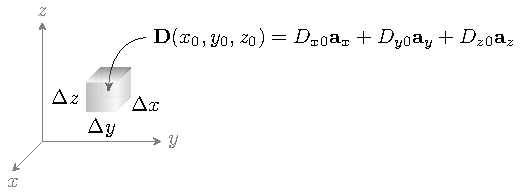
\includegraphics{figGaussDifferentialVolumeCartesianCoordinates}
\caption{انتہائی چھوٹی حجم پر گاؤس کے قانون کا اطلاق}
\label{شکل_گاؤس_چھوٹی_حجم_پر_اطلاق}
\end{figure}

ہمیں \عددیء{\kvec{D}} کی قیمت ڈبیہ کے  وسط میں معلوم ہے۔\اصطلاح{ٹیلر تسلسل}\فرہنگ{ٹیلر تسلسل}\حاشیہب{Taylor series}\فرہنگ{Taylor series} کے مطابق کسی بھی تفاعل جس کی قیمت نقطہ \عددیء{a} پر معلوم ہو کو اس نقطے کے قریبی نقطوں پر
\begin{align*}
f(x+a)=f(a)+\frac{1}{1!}(x-a)f'(a)+\frac{1}{2!}(x-a)^2 f''(a)+\cdots
\end{align*}
سے حاصل کیا جا سکتا ہے۔ڈبیہ کے وسط میں نقطہ \عددیء{N(x_0,y_0,z_0)} پر 
\begin{align*}
\kvec{D}(x_0,y_0,z_0)=D_{x0}\ax+D_{y0}\ay+D_{z0}\az
\end{align*}
کی قیمت سے وسط سے \عددیء{+\tfrac{\Delta x}{2}} فاصلے پر  ڈبیہ کے سامنے سطح پر  \عددیء{D_x} ٹیلر تسلسل سے یوں حاصل کیا جا سکتا ہے۔
\begin{align*}
D_{x,\textrm{سامنے}}&=D_{x0}+\frac{1}{1!}\frac{\Delta x}{2} \frac{\partial D_x}{\partial x}+\frac{1}{2!}\left[\frac{\Delta x}{2}\right]^2 \frac{\partial^2 D_x}{\partial x^2}\cdots\\
&\overset{.}{=}D_{x0}+\frac{\Delta x}{2} \frac{\partial D_x}{\partial x}
\end{align*}
جہاں دوسرے قدم پر تسلسل کے صرف پہلے دو اجزاء لئے گئے ہیں۔تفاعل  کے ایک سے زیادہ متغیرات \عددیء{x}، \عددیء{y} اور \عددیء{z} ہیں لہٰذا تسلسل میں جزوی تفرق\حاشیہب{partial differential} کا استعمال کیا گیا ۔

یوں
\begin{align*}
\int\limits_{\textrm{سامنے}} &\overset{.}{=} \left(D_{x0}+\frac{\Delta x}{2} \frac{\partial D_x}{\partial x} \right) \Delta y \Delta z
\end{align*}
حاصل ہوتا ہے۔

بند سطح کی سمت باہر جانب ہوتی ہے لہٰذا پچلی سطح \عددیء{-\Delta y \Delta z \ax} ہے اور یوں ڈبیہ کی پچلی سطح کے  لئے
\begin{align*}
\int\limits_{\textrm{پیچے}} &\overset{.}{=} \kvec{D}_{\textrm{پیچے}} \cdot \Delta \kvec{S}_{\textrm{پیچے}}\\
&\overset{.}{=}\left(D_x \ax+D_y\ay+D_z\az \right)_{\textrm{پیچے}} \cdot \left(-\Delta y \Delta z \ax\right)\\
&\overset{.}{=} -D_{x,\textrm{پیچے}} \Delta y \Delta z
\end{align*}
لکھا جا سکتا ہے جہاں وسط سے \عددیء{-\tfrac{\Delta x}{2}} فاصلے پر  ڈبیہ کی پچلی  سطح پر  \عددیء{D_x} ٹیلر تسلسل سے
\begin{align*}
D_{x,\textrm{پیچے}}&=D_{x0}-\frac{\Delta x}{2} \frac{\partial D_x}{\partial x}
\end{align*}
حاصل ہوتا ہے۔یوں
\begin{align*}
\int\limits_{\textrm{پیچے}} &\overset{.}{=} -\left(D_{x0}-\frac{\Delta x}{2} \frac{\partial D_x}{\partial x} \right) \Delta y \Delta z
\end{align*}
اور
\begin{align*}
\int\limits_{\textrm{سامنے}}+\int\limits_{\textrm{پیچے}}&\overset{.}{=}  \left(D_{x0}+\frac{\Delta x}{2} \frac{\partial D_x}{\partial x} \right) \Delta y \Delta z -\left(D_{x0}-\frac{\Delta x}{2} \frac{\partial D_x}{\partial x} \right) \Delta y \Delta z\\
&\overset{.}{=} \frac{\partial D_x}{\partial x} \Delta x \Delta y \Delta z
\end{align*}

حاصل ہوتا ہے۔اسی عمل کو دہراتے ہوئے بائیں اور دائیں سطحوں کے لئے
\begin{align*}
\int\limits_{\textrm{بائیں}}+\int\limits_{\textrm{دائیں}}\overset{.}{=}  \frac{\partial D_y}{\partial y} \Delta x \Delta y \Delta z
\end{align*}
اور اوپر، نیچے سطحوں کے لئے
\begin{align*}
\int\limits_{\textrm{اوپر}}+\int\limits_{\textrm{نیچے}}\overset{.}{=}  \frac{\partial D_z}{\partial z} \Delta x \Delta y \Delta z
\end{align*}
حاصل ہوتا ہے۔اس طرح 
\begin{align}\label{مساوات_گاؤس_کارتیسی_محدد_چھوٹی_حجم}
\oint\limits_{S}\kvec{D}\cdot \dif \kvec{S}=Q\overset{.}{=} \left( \frac{\partial D_x}{\partial x}+\frac{\partial D_y}{\partial y}+\frac{\partial D_z}{\partial z} \right)\Delta x \Delta y \Delta z 
\end{align}
حاصل ہوتا ہے۔

اس مساوات کے تحت کسی بھی نقطے پر انتہائی چھوٹی حجم \عددیء{\Delta h} میں چارج تقریباً
\begin{align}
Q\overset{.}{=} \left( \frac{\partial D_x}{\partial x}+\frac{\partial D_y}{\partial y}+\frac{\partial D_z}{\partial z} \right)\Delta h
\end{align}
کے برابر ہے۔حجم کی جسامت جتنی کم کی جائے جواب اتنا زیادہ درست ہو گا۔اگلے حصے میں حجم کو کم کرتے کرتے نقطہ نما بنا دیا جائے گا۔ایسی صورت میں مندرجہ بالا مساوات مکمل طور صحیح جواب مہیا کرے گا۔
%==========
\ابتدا{مثال}
اگر \عددیء{\kvec{D}=2x\ax+3y\ay+5\az \, \si{\coulomb / \meter\squared}} ہو تب کارتیسی محدد کے مرکز پر \عددیء{\SI{e-9}{\meter \cubed}} کے انتہائی چھوٹی حجم میں چارج حاصل کریں۔

حل:
\begin{align*}
\frac{\partial D_x}{\partial x}+\frac{\partial D_y}{\partial y}+\frac{\partial D_z}{\partial z} =2+3+0
\end{align*}
سے اس حجم میں \عددیء{5 \times 10^{-9}=\SI{5}{\nano \coulomb}} چارج  پایا جائے گا۔
\انتہا{مثال}
%========================

\حصہ{پھیلاو}
مساوات \حوالہ{مساوات_گاؤس_کارتیسی_محدد_چھوٹی_حجم} میں حجم  کو اتنا کم کرتے ہوئے کہ اس کو صفر تصور کرنا ممکن ہو
\begin{align*}
\frac{\partial D_x}{\partial x}+\frac{\partial D_y}{\partial y}+\frac{\partial D_z}{\partial z}=\lim_{\Delta h \to 0}\frac{\oint\limits_{S}\kvec{D}\cdot \dif \kvec{S}}{\Delta h}=\lim_{\Delta h \to 0} \frac{Q}{\Delta h}
\end{align*}
لکھا جا سکتا ہے۔چارج فی حجم کو حجمی کثافت کہتے ہیں۔یوں مساوات کا دایاں بازو نقطے پر حجمی کثافت \عددیء{\rho_h} دیتا ہے۔اس طرح اس مساوات سے دو مساوات حاصل کئے جا سکتے ہیں یعنی
\begin{align}\label{مساوات_گاؤس_میکسویل_پھیلاو_مساوات}
\frac{\partial D_x}{\partial x}+\frac{\partial D_y}{\partial y}+\frac{\partial D_z}{\partial z}=\rho_h
\end{align}
اور 
\begin{align}\label{مساوات_گاؤس_پھیلاو_کی_تعریف}
\frac{\partial D_x}{\partial x}+\frac{\partial D_y}{\partial y}+\frac{\partial D_z}{\partial z}=\lim_{\Delta h \to 0}\frac{\oint\limits_{S}\kvec{D}\cdot \dif \kvec{S}}{\Delta h}
\end{align}
مساوات \حوالہ{مساوات_گاؤس_میکسویل_پھیلاو_مساوات} میکس ویل کی پہلی مساوات ہے جبکہ مساوات \حوالہ{مساوات_گاؤس_پھیلاو_کی_تعریف} سمتیہ \عددیء{\kvec{D}} کا \اصطلاح{پھیلاو}\فرہنگ{پھیلاو}\حاشیہب{divergence}\فرہنگ{divergence} بیان کرتا ہے۔اس مساوات کا دایاں بازو پھیلاو کی تعریف جبکہ اس کا بایاں بازو پھیلاو حاصل کرنے کا طریقہ دیتا ہے۔یوں کارتیسی محدد میں 
\begin{align}\label{مساوات_گاؤس_کارتیسی_محدد_پھیلاو_کی_مساوات}
\frac{\partial D_x}{\partial x}+\frac{\partial D_y}{\partial y}+\frac{\partial D_z}{\partial z} \quad \textrm{کارتیسی محدد میں پھیلاو کی مساوات}
\end{align}
سے سمتیہ \عددیء{\kvec{D}} کا پھیلاو حاصل کیا جاتا ہے۔

انجنیئرنگ  کے شعبے میں ایسے کئی مسئلے پائے جاتے ہیں جن  میں چھوٹی سی حجم  کو گھیرنے والے بند سطح پر کسی سمتیہ \عددیء{\kvec{K}} کا  \عددیء{\oint_{S}\kvec{K}\cdot \dif \kvec{S}} درکار ہو۔گزشتہ حصے میں سمتیہ \عددیء{\kvec{D}} کے لئے ایسا ہی کیا گیا۔غور کرنے سے معلوم ہوتا ہے کہ ایسا کرتے ہوئے  \عددیء{\kvec{D}} کی جگہ \عددیء{\kvec{K}} لکھا جا سکتا ہے جس سے 
\begin{align}\label{مساوات_گاؤس_کارتیسی_پھیلاو_کی_تعریف}
\frac{\partial K_x}{\partial x}+\frac{\partial K_y}{\partial y}+\frac{\partial K_z}{\partial z}=\lim_{\Delta h \to 0}\frac{\oint\limits_{S}\kvec{K}\cdot \dif \kvec{S}}{\Delta h}
\end{align}
حاصل ہوتا۔سمتیہ \عددیء{\kvec{K}} پانی کا بہاو، ایٹموں کی رفتار یا سلیکان کی پتری میں درجہ حرارت ہو سکتا ہے۔ہم \عددیء{\kvec{K}} کو سمتی بہاو کی کثافت تصور کریں گے۔مندرجہ بالا مساوات  \عددیء{\kvec{K}} کا پھیلاو بیان کرتا ہے۔پھیلاو کے عمل سے مراد مساوات کے بائیں بازو کا عمل ہے  جبکہ مساوات کا دایاں بازو اس کی تعریف بیان کرتا ہے جس کے تحت

\ابتدا{قانون}
کسی بھی سمتی کثافتی بہاو کے \اصطلاح{پھیلاو} سے مراد کسی  چھوٹی حجم کو صفر کرتے ہوئے اس  سے خارج کُل بہاو فی اکائی حجم ہے۔ 
\انتہا{قانون}

یہ ضروری ہے کہ آپ کو پھیلاو کی تعریف کی سمجھ ہو۔یاد رہے کہ پھیلاو کا عمل سمتیہ پر کیا جاتا ہے جبکہ اس سے حاصل جواب مقداری ہوتا ہے۔کسی نقطے پر چھوٹی حجم سے باہر جانب کل بہاو فی چھوٹی حجم کو پھیلاو کہتے ہیں۔پھیلاو کی کوئی سمت نہیں ہوتی۔پھیلاو کی تعریف جانتے ہوئے کئی مرتبہ بغیر قلم اٹھائے جواب حاصل کیا جا سکتا ہے۔اسی نوعیت کے چند مسئلوں پر اب غور کرتے ہیں۔

پانی سے بھری بالٹی میں پانی میں ڈوبے کسی بھی نقطے پر پانی کی رفتار کا پھیلاو صفر ہو گا چونکہ اس نقطے سے نہ پانی باہر نکل رہا ہے اور نا ہی اس میں داخل ہو رہا ہے۔اسی طرح دریا میں پانی میں دھوبے نقطے پر بھی پانی کے رفتار کا پھیلاو صفر ہو گا چونکہ ایسے نقطے سے جتنا پانی نکلتا ہے، اتنا ہی پانی اس میں داخل ہوتا ہے۔البتہ اگر بھری بالٹی کے تہہ میں سوراخ کر دیا جائے  تو جب تک نقطہ پانی میں دھوبا رہے اس وقت تک یہاں پھیلاو صفر رہے  گا البتہ جیسے ہی نقطہ پانی سے نمودار ہونے لگے یہاں مثبت پھیلاو پایا جائے گا اور جب نقطہ پانی سے مکمل طور باہر آ جائے تب ایک بار پھر یہاں پھیلاو صفر ہو جائے گا۔جتنی دیر نقطہ پانی کی سطح سے باہر نمودار ہو رہا ہوتا ہے اتنی دیر اس نقطے سے پانی کی انخلا پائی جاتی ہے جس کی وجہ سے یہاں پھیلاو پایا جاتا ہے۔

ایک اور دلچسپ مثال سائکل کے ٹائر میں ہوا کی ہے۔اگر ٹائر پنکچر ہو جائے اور اس سے ہوا نکلنی شروع ہو جائے تو ٹائر میں کسی بھی نقطے پر سمتی رفتار کا پھیلاو پایا جائے گا چونکہ کسی بھی نقطے پر دیکھا جائے تو یہاں سے ہوا پھیلتے ہوئے خارج ہو گا۔یوں مثبت پھیلاو سے مراد نقطے سے انخلا جبکہ منفی پھیلاو سے مراد نقطے میں داخل ہونا ہے۔ 

ریاضیاتی عمل کو بیان کرنے کے لئے عموماً علامت استعمال کی جاتی ہے۔یوں جمع کے لئے \عددیء{+}، ضرب کے لئے \عددیء{\times} اور تکملہ کے لئے \عددیء{\int} استعمال کئے جاتے ہیں۔آئیں ایک نئی علامت  جسے \اصطلاح{نیبلا}\فرہنگ{نیبلا}\حاشیہب{nabla, del}\فرہنگ{nabla} کہتے اور \عددیء{\nabla} سے ظاہر کرتے ہیں سیکھیں۔تصور کریں کہ
\begin{align}\label{مساوات-گاؤس_نیبلا}
\nabla = \frac{\partial }{\partial x}\ax+\frac{\partial }{\partial y}\ay+\frac{\partial }{\partial z}\az
\end{align}
لکھا جاتا ہے جہاں مقداری متغیرہ \عددیء{f} کے سامنے لکھنے سے مراد
\begin{align}\label{مساوات_گاؤس_ڈیل_مقداری}
\nabla f = \frac{\partial f}{\partial x}\ax+\frac{\partial f}{\partial y}\ay+\frac{\partial f}{\partial z}\az
\end{align}
جبکہ سمتیہ \عددیء{\kvec{K}} کے ساتھ نقطہ ضرب سے مراد
\begin{gather}
\begin{aligned}
\nabla \cdot \kvec{K}&=\left(\frac{\partial }{\partial x}\ax+\frac{\partial }{\partial y}\ay+\frac{\partial }{\partial z}\az \right) \cdot \left (K_x \ax+K_y \ay+K_z \az \right)\\
&=\frac{\partial K_x}{\partial x}+\frac{\partial K_y}{\partial y}+\frac{\partial K_z}{\partial z}
\end{aligned}
\end{gather}
لیا جاتا ہے۔یہ علامت انجنیئرنگ  کے شعبے میں انتہائی مقبول ہے۔اسے استعمال کرتے ہوئے پھیلاو کو \عددیء{\nabla \cdot \kvec{D}}  لکھا جا سکتا ہے جہاں
\begin{align}\label{مساوات_گاوس_پھیلاو}
\nabla \cdot \kvec{D}=\frac{\partial D_x}{\partial x}+\frac{\partial D_y}{\partial y}+\frac{\partial D_z}{\partial z}
\end{align}
کے برابر ہے۔پھیلاو کے عمل کو ہم اسی علامت سے ظاہر کریں گے۔مساوات \حوالہ{مساوات_گاؤس_میکسویل_پھیلاو_مساوات} یعنی میکس ویل کی پہلی مساوات اب یوں لکھی جا سکتی ہے۔
\begin{align}
\nabla \cdot \kvec{D}=\rho_h \quad \textrm{میکس ویل کی پہلی مساوات}
\end{align}
میکس ویل کی پہلی مساوات درحقیقت گاؤس کے قانون کی تفرق\حاشیہب{differential} شکل ہے۔اسی طرح گاؤس کا قانون میکس ویل مساوات کی تکمل\حاشیہب{integral} شکل ہے۔

مساوات \حوالہ{مساوات_گاؤس_ڈیل_مقداری} کے طرز پر مساوات صفحہ \حوالہصفحہ{مساوات_توانائی_ڈھلان_تعریف_پ} پر دیا گیا ہے۔
%=================
\حصہ{نلکی محدد میں پھیلاو کی مساوات}
حصہ \حوالہ{حصہ_گاؤس_چھوٹی_حجم_گاؤس_کا_اطلاق} میں کارتیسی محدد استعمال کرتے ہوئے چھوٹی حجم پر گاؤس کے قانون کے اطلاق سے پھیلاو کی مساوات حاصل کی گئی۔اس حصے میں نلکی محدد استعمال کرتے ہوئے شکل میں دکھائے چھوٹی حجم کو استعمال کرتے ہوئے پھیلاو کی مساوات حاصل کی جائے گی۔شکل کو دیکھتے ہوئے
\begin{align*}
\Delta_{S\textrm{سامنے}}&=-\Delta \rho \Delta z \aphi\\
\Delta_{S\textrm{پیچے}}&=+\Delta \rho \Delta z \aphi\\
\Delta_{S\textrm{بائیں}}&=-\left(\rho-\frac{\Delta \rho}{2} \right) \Delta \phi \Delta z \arho\\
\Delta_{S\textrm{دائیں}}&=+\left(\rho+\frac{\Delta \rho}{2} \right) \Delta \phi \Delta z \arho\\
\Delta_{S\textrm{اوپر}}&=+\rho \Delta \phi \Delta \rho \az\\
\Delta_{S\textrm{نیچے}}&=-\rho \Delta \phi \Delta \rho \az\\
\end{align*}
لکھا جا سکتا ہے۔کارتیسی محدد میں آمنے سامنے رقبے برابر  تھے۔نلکی محدد میں بائیں اور دائیں رقبے برابر نہیں ہیں۔اس فرق کی بنا پر نلکی محدد میں پھیلاو کی مساوات قدر مختلف حاصل ہو گی۔چھوٹی حجم کے وسط میں
\begin{align}
\kvec{D}=D_{\rho 0} \arho+D_{\phi 0} \aphi+D_{z 0} \az
\end{align}
کے برابر ہے جس سے ٹیلر تسلسل کی مدد سے
\begin{align*}
\kvec{D}_{\textrm{سامنے}}&=\left( D_{\phi 0}-\frac{\Delta \phi}{2}\frac{\partial D_{\phi}}{\partial \phi} \right) \aphi\\
\kvec{D}_{\textrm{پیچے}}&=\left( D_{\phi 0}+\frac{\Delta \phi}{2}\frac{\partial D_{\phi}}{\partial \phi} \right)\aphi \\
\kvec{D}_{\textrm{بائیں}}&=\left( D_{\rho 0}-\frac{\Delta \rho}{2}\frac{\partial D_{\rho}}{\partial \rho} \right) \arho\\
\kvec{D}_{\textrm{دائیں}}&=\left( D_{\rho 0}+\frac{\Delta \rho}{2}\frac{\partial D_{\rho}}{\partial \rho} \right) \arho\\
\kvec{D}_{\textrm{اوپر}}&=\left( D_{z 0}+\frac{\Delta z}{2}\frac{\partial D_{z}}{\partial z} \right) \az\\
\kvec{D}_{\textrm{نیچے}}&=\left( D_{z 0}-\frac{\Delta z}{2}\frac{\partial D_{z}}{\partial z} \right) \az
\end{align*}
لکھا جا سکتا ہے۔یوں
\begin{align*}
\int \limits_{\textrm{سامنے}}+\int\limits_{\textrm{پیچے}}=\frac{\partial D_{\phi}}{\partial \phi} \Delta \rho \Delta \phi \Delta z
\end{align*}
حاصل ہوتا ہے۔اسی طرح
\begin{align*}
\int \limits_{\textrm{بائیں}}+\int \limits_{\textrm{دائیں}}=\left(D_{\rho 0} +\rho \frac{\partial D_{\rho}}{\partial \rho} \right) \Delta \rho \Delta \phi \Delta z
\end{align*}
حاصل ہوتا ہے جسے
\begin{align*}
\int \limits_{\textrm{بائیں}}+\int \limits_{\textrm{دائیں}}=\frac{\partial (\rho D_{\rho})}{\partial \rho}  \Delta \rho \Delta \phi \Delta z
\end{align*}
بھی لکھا جا سکتا ہے۔ایسا لکھتے وقت یاد رہے کہ نقطہ \عددیء{N(\rho_0 , \phi_0 , z_0)} پر
\begin{align*}
\eval{\frac{\partial (\rho D_{\rho})}{\partial \rho}}_{N}=\eval{D_{\rho}+\rho \frac{\Delta D_{\rho}}{\Delta \rho}}_{N}=D_{\rho 0} +\rho \frac{\partial D_{\rho}}{\partial \rho}
\end{align*}
کے برابر ہے۔اسی طرح
\begin{align*}
\int \limits_{\textrm{اوپر}}+\int\limits_{\textrm{نیچے}}=\rho \frac{\partial D_{z}}{\partial z} \Delta \rho \Delta \phi \Delta z
\end{align*}
حاصل ہوتا ہے۔ان تمام کو استعمال کرتے ہوئے
\begin{align*}
\oint\limits_{S} \kvec{D}_S \cdot \dif \kvec{S}=\left(\frac{\partial (\rho D_{\rho})}{\partial \rho}+\frac{\partial D_{\phi}}{\partial \phi}  + \rho \frac{\partial D_{z}}{\partial z}   \right)\Delta \rho \Delta \phi \Delta z
\end{align*}
ملتا ہے۔چھوٹی حجم \عددیء{\Delta h = \rho \Delta \rho \Delta \phi \Delta z} کے استعمال سے
\begin{align}\label{مساوات_گاؤس_نلکی_پھیلاو_کی_تعریف}
\frac{1}{\rho}\frac{\partial (\rho D_{\rho})}{\partial \rho}+\frac{1}{\rho}\frac{\partial D_{\phi}}{\partial \phi}  +  \frac{\partial D_{z}}{\partial z}=\lim_{\Delta h \to 0} \frac{\oint\limits_{S} \kvec{D}_S \cdot \dif \kvec{S}}{\Delta h}
\end{align}
حاصل ہوتا ہے۔مساوات \حوالہ{مساوات_گاؤس_کارتیسی_پھیلاو_کی_تعریف} کا دایاں بازو پھیلاو کی تعریف بیان کرتا ہے جس کے ساتھ موازنہ کرنے سے آپ دیکھ سکتے ہیں کہ مساوات \حوالہ{مساوات_گاؤس_نلکی_پھیلاو_کی_تعریف} نلکی محدد میں پھیلاو  دیتا ہے۔

آپ دیکھ سکتے ہیں کہ نلکی محدد میں پھیلاو کی مساوات سادہ شکل نہیں رکھتی۔مساوات \حوالہ{مساوات-گاؤس_نیبلا} میں دی گئی \عددیء{\nabla} کو استعمال کرتے ہوئے نلکی محدد میں پھیلاو کی مساوات ہرگز حاصل نہیں کی جا سکتی ہے۔اس کے باوجود نلکی محدد میں بھی پھیلاو کے عمل کو \عددیء{\nabla \cdot \kvec{D}} سے ہی ظاہر کیا جا سکتا ہے جہاں اس سے مراد
\begin{align}
\nabla \cdot \kvec{D}=\frac{1}{\rho}\frac{\partial (\rho D_{\rho})}{\partial \rho}+\frac{1}{\rho}\frac{\partial D_{\phi}}{\partial \phi}  +  \frac{\partial D_{z}}{\partial z}
\end{align}
لیا جاتا ہے۔
 

\حصہ{پھیلاو کی عمومی مساوات}\شناخت{حصہ_گاوس_عمومی_پھیلاو}
کارتیسی محدد میں چھوٹی حجم کے آمنے سامنے اطراف کا رقبہ برابر ہوتا ہے جس سے پھیلاو کی مساوات آسانی سے حاصل ہوتی ہے۔نلکی محدد میں چھوٹی حجم کے رداسی سمت کے آمنے سامنے رقبے مختلف ہوتے ہیں جن کا خصوصی خیال رکھتے ہوئے پھیلاو کی قدر مشکل مساوات گزشتہ حصے میں حاصل کی گئی۔اس حصے میں پھیلاو کی مساوات حاصل کرنے کا ایسا طریقہ دیکھتے ہیں جسے استعمال کرتے ہوئے پھیلاو کی عمومی مساوات حاصل کی جا سکتی ہے جو تمام محدد کے لئے کارآمد ہے۔

کارتیسی محدد کے متغیرات \عددیء{(x,y,z)} جبکہ نلکی محدد کے  \عددیء{(\rho, \phi,z )} اور کروی محدد  کے متغیرات \عددیء{(r,\theta,\phi)} ہیں۔اس حصے میں \اصطلاح{عمومی محدد}\فرہنگ{محدد!عمومی}\حاشیہب{generalized coordinates}\فرہنگ{coordinates!generalized}  استعمال کیا جائے گا جس کے متغیرات \عددیء{(u,v,w)}  اور  تین عمودی اکائی سمتیات \عددیء{(\au, \av, \aw)} ہیں۔عمومی محدد کسی بھی محدد کے لئے استعمال کیا جا سکتا ہے۔یوں اگر اسے کارتیسی محدد کے لئے استعمال کیا جا رہا ہو تب \عددیء{(u,v,w)}  سے مراد \عددیء{(x,y,z)} ہو گا۔
 
شکل میں عمومی محدد استعمال کرتے ہوئے چھوٹی حجم دکھائی گئی ہے۔عمومی محدد کے تین اطراف
\begin{align*}
\dif L_1 &= k_1 \dif u \\
\dif L_2 &= k_2 \dif v \\
\dif L_3 &= k_3 \dif w 
\end{align*}
ہیں۔کارتیسی محدد میں \عددیء{k_1=k_2=k_3=1} کے برابر لیا جائے گا اور یوں \عددیء{\dif L_1=\dif x } کے برابر ہو گا۔نلکی محدد میں
\begin{gather}
\begin{aligned}\label{مساوات_گاؤس_نلکی_اطراف_کے_مستقل}
k_1&=1\\
k_2&=\rho\\
k_3&=1
\end{aligned}
\end{gather}
جبکہ کروی محدد میں
\begin{gather}
\begin{aligned}\label{مساوات_گاؤس_کروی_اطراف_کے_مستقل}
k_1&=1\\
k_2&=r\\
k_3&=r \sin \theta
\end{aligned}
\end{gather}
کے برابر ہیں۔اسی طرح تین سمتی رقبے
\begin{align*}
& \dif L_2 \dif L_3 \au\\
&\dif L_1 \dif L_3 \av\\
&\dif L_1 \dif L_2 \aw
\end{align*}
ہوں گے۔

گزشتہ حصوں میں چھوٹی حجم کے آمنے سامنے سطحوں پر بہاو حاصل کرتے وقت پہلے  ان سطحوں پر \عددیء{\kvec{D}} کی قیمت اور ان سطحوں کے رقبے حاصل کئے گئے جن کے نقطہ ضرب سے بہاو حاصل کیا گیا۔یہاں چھوٹی حجم کے وسط میں تین اکائی سمتیات کی سمت میں بہاو سے ٹیلر تسلسل کے استعمال سے حجم کے سطحوں پر بہاو حاصل کیا جائے گا۔حجم کے وسط میں تین اکائی سمتیات کے رخ میں سطحوں پر بہاو
\begin{align*}
& \dif L_2 \dif L_3  D_{u0}\\
& \dif L_1 \dif L_3  D_{v0}\\
& \dif L_1 \dif L_2  D_{w0}
\end{align*}
ہے۔ٹیلر تسلسل سے سامنے اور پیچے سطحوں پر ان مساوات سے
\begin{align*}
\dif L_2 \dif L_3  D_{u0} &+\frac{1}{2}\frac{\partial }{\partial u} ( \dif L_2 \dif L_3  D_{u})\dif u \quad \textrm{سامنے}\\
-\dif L_2 \dif L_3  D_{u0} &+\frac{1}{2}\frac{\partial }{\partial u} ( \dif L_2 \dif L_3  D_{u})\dif u \quad \textrm{پیچے}
\end{align*}
یعنی
\begin{align*}
k_2 k_3 \dif v \dif w  D_{u0} &+\frac{1}{2}\frac{\partial }{\partial u} ( k_2 k_3  D_{u})\dif u  \dif v \dif w\quad \textrm{سامنے}\\
-k_2 k_3 \dif v \dif w  D_{u0} &+\frac{1}{2}\frac{\partial }{\partial u} ( k_2 k_3  D_{u})\dif u  \dif v \dif w\quad \textrm{پیچے}
\end{align*}
لکھتے ہوئے دونوں سطحوں پر بہاو کا مجموعہ
\begin{align*}
\frac{\partial }{\partial u} ( k_2 k_3  D_{u})\dif u  \dif v \dif w
\end{align*}
حاصل ہوتا ہے۔اسی طرح بائیں اور دائیں سطحوں پر کل
\begin{align*}
\frac{\partial }{\partial v} ( k_1 k_3  D_{v})\dif u  \dif v \dif w
\end{align*}
اور اوپر، نیچے کا مجموعہ
\begin{align*}
\frac{\partial }{\partial w} ( k_1 k_2  D_{w})\dif u  \dif v \dif w
\end{align*}
حاصل ہوتا ہے۔چھوٹی حجم
\begin{align*}
\dif h &= \dif L_1 \dif L_2 \dif L_3 \\
&= k_1 k_2 k_3 \dif u \dif v \dif w
\end{align*}
لکھتے ہوئے گاؤس کے قانون سے
\begin{align*}
\oint\limits_{S} \kvec{D} \cdot \dif \kvec{S}=\left[\frac{\partial }{\partial u} ( k_2 k_3  D_{u})+\frac{\partial }{\partial v} ( k_1 k_3  D_{v})+\frac{\partial }{\partial w} ( k_1 k_2  D_{w}) \right]\dif u  \dif v \dif w 
\end{align*}
یعنی
\begin{align*}
\frac{1}{k_1 k_2 k_3}\left[\frac{\partial }{\partial u} ( k_2 k_3  D_{u})+\frac{\partial }{\partial v} ( k_1 k_3  D_{v})+\frac{\partial }{\partial w} ( k_1 k_2  D_{w}) \right] =\lim_{\dif h \to 0}\frac{\oint\limits_{S} \kvec{D} \cdot \dif \kvec{S}}{\dif h}
\end{align*}
حاصل ہوتا ہے۔اس مساوات کا دایاں بازو پھیلاو کی تعریف ہے۔یوں پھیلاو کی عمومی مساوات
\begin{align}\label{مساوات_گاؤس_پھیلاو_کی_عمومی_مساوات}
\nabla \cdot \kvec{D}=\frac{1}{k_1 k_2 k_3}\left[\frac{\partial }{\partial u} ( k_2 k_3  D_{u})+\frac{\partial }{\partial v} ( k_1 k_3  D_{v})+\frac{\partial }{\partial w} ( k_1 k_2  D_{w}) \right] 
\end{align}
حاصل ہوتی ہے۔
%==============
\ابتدا{مثال}
مساوات \حوالہ{مساوات_گاؤس_پھیلاو_کی_عمومی_مساوات} سے  نلکی اور کروی محدد میں پھیلاو کی مساوات حاصل کریں۔

حل: \عددیء{u,v,w} کی جگہ \عددیء{\rho, \phi, z} اور مساوات \حوالہ{مساوات_گاؤس_نلکی_اطراف_کے_مستقل} کے استعمال سے  نلکی محدد میں پھیلاو
\begin{gather}
\begin{aligned}
\nabla \cdot \kvec{D}&=\frac{1}{\rho}\left[\frac{\partial }{\partial \rho} ( \rho  D_{\rho})+\frac{\partial }{\partial \phi} (   D_{\phi})+\frac{\partial }{\partial z} ( \rho  D_{z}) \right]\\
&=\frac{1}{\rho}\frac{\partial }{\partial \rho} ( \rho  D_{\rho})+\frac{1}{\rho}\frac{\partial }{\partial \phi} (   D_{\phi})+\frac{\partial }{\partial z} ( D_{z}) \quad \textrm{نلکی محدد میں پھیلاو کی مساوات}
\end{aligned}
\end{gather}
حاصل ہوتا ہے۔اسی طرح  \عددیء{u,v,w} کی جگہ \عددیء{r,\theta,\phi} اور مساوات \حوالہ{مساوات_گاؤس_کروی_اطراف_کے_مستقل} کے استعمال سے کروی محدد میں پھیلاو
\begin{gather}
\begin{aligned}
\nabla \cdot \kvec{D}&=\frac{1}{r^2 \sin \theta}\left[\frac{\partial }{\partial r} (r^2 \sin \theta  D_{r})+\frac{\partial }{\partial \theta} ( r \sin \theta  D_{\theta})+\frac{\partial }{\partial \phi} ( r  D_{\phi}) \right]\\
&=\frac{1}{r^2 }\frac{\partial }{\partial r} (r^2   D_{r})+\frac{1}{r \sin \theta }\frac{\partial }{\partial \theta} (\sin \theta  D_{\theta})+\frac{1}{r \sin \theta }\frac{\partial }{\partial \phi} (  D_{\phi})\quad \textrm{کروی محدد میں پھیلاو کی مساوات}
\end{aligned}
\end{gather}
حاصل ہوتا ہے۔
\انتہا{مثال}
%=================
\حصہ{مسئلہ پھیلاو}
صفحہ \حوالہصفحہ{مساوات_گاؤس_چھوٹی_ڈبیہ_کارتیسی_محدد} پر مساوات \حوالہ{مساوات_گاؤس_چھوٹی_ڈبیہ_کارتیسی_محدد} میں
\begin{align*}
\nabla \cdot \kvec{D}=\rho_h
\end{align*}
لکھتے ہوئے
\begin{align}
\oint\limits_{S} \kvec{D} \cdot \dif \kvec{S}=\int\limits_{h} \nabla \cdot \kvec{D} \dif h
\end{align}
لکھا جا سکتا ہے جو \اصطلاح{مسئلہ پھیلاو}\فرہنگ{مسئلہ پھیلاو}\حاشیہب{divergence theorem}\فرہنگ{divergence theorem} بیان کرتا ہے۔اگرچہ ہم  نے اس مسئلے کو برقی بہاو \عددیء{\kvec{D}} کے لئے حاصل کیا حقیقت میں یہ ایک عمومی نتیجہ ہے جو کسی بھی تین درجی تکملہ کو دو درجی تکملہ اور دو درجی تکملہ کو تین درجی تکملہ میں تبدیل کرتا ہے۔مسئلہ پھیلاو کو یوں بیان کیا جا سکتا ہے

کسی بھی بند سطح پر  سمتیہ کے عمودی حصے کا تکملہ بند حجم میں اسی سمتیہ کے پھیلاو کے تکملہ کے برابر ہوتا ہے۔\حاشیہط{فاصلہ رکھیں}

\begin{figure}
\centering
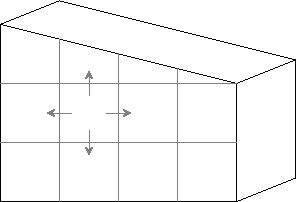
\includegraphics{figGaussDiversionAsSurfaceIntegral}
\caption{بند سطح پر سمتیہ کا عمودی حصے کا تکملہ بند حجم میں سمتیہ کے تکملہ کے برابر ہوتا ہے۔}
\label{شکل_گاؤس_پھیلاو_بطور_سطحی_تکلہ}
\end{figure}

مسئلہ پھیلاو کی سمجھ شکل \حوالہ{شکل_گاؤس_پھیلاو_بطور_سطحی_تکلہ} کی مدد سے با آسانی ممکن ہے۔جیسے شکل میں دکھایا گیا ہے کہ کسی بھی چھوٹی حجم سے بہاو قریبی چھوٹی حجم  کی منفی بہاو ثابت ہوتی ہے لہٰذا دونوں کا مجموعی بہاو  حاصل کرتے ہوئے ان کے درمیانی دیوار  پر بہاو رد کیا جائے گا۔یہی سلسلہ تمام حجم پر لاگو کرتے ہوئے ظاہر ہے کہ پوری حجم سے بہاو کے حصول میں اندرونی تمام دیواروں پر بہاو کا کوئی کردار نہیں ہوتا اور صرف بیرونی سطح پر بہاو سے ہی جواب حاصل کیا جا سکتا ہے۔
%==============

\ابتدا{مثال}
نقطہ چارج کے \عددیء{\kvec{D}} سے پھیلاو کی مساوات سے مختلف مقامات پر کثافت چارج \عددیء{\rho_h} حاصل کریں۔

حل:کروی محدد کے مرکز پر نقطہ چارج کا
\begin{align*}
\kvec{D}=\frac{Q}{4\pi r^2} \ar
\end{align*}
ہوتا ہے۔کروی محدد میں پھیلاو کی مساوات کے تحت
\begin{align*}
\nabla \cdot \kvec{D}=\frac{1}{r^2 }\frac{\partial }{\partial r} (r^2   D_{r})+\frac{1}{r \sin \theta }\frac{\partial }{\partial \theta} (\sin \theta  D_{\theta})+\frac{1}{r \sin \theta }\frac{\partial }{\partial \phi} (  D_{\phi}) 
\end{align*}
کے برابر ہے۔چونکہ \عددیء{D_{\theta}} اور \عددیء{D_{\phi}} صفر کے برابر ہیں لہٰذا مندرجہ بالا مساوات سے
\begin{align*}
\nabla \cdot \kvec{D}=\frac{1}{r^2 }\frac{\partial }{\partial r} (r^2 \frac{Q}{4\pi r^2}  )=\left\{
\begin{array}{l  l}
0 &\quad r> 0\\
\infty & \quad r=0
\end{array}
\right.
\end{align*}
حاصل ہوتا ہے جس کے تحت مرکز کے علاوہ تمام خلاء میں کوئی چارج نہیں پایا جاتا۔مرکز پر لامحدود کثافت کا چارج پایا جاتا ہے۔یاد رہے کہ نقطہ چارج سے مراد ایسا چارج ہے جس کا حجم صفر ہو۔ایسی صورت میں اس نقطے پر نقطہ چارج کی کثافت لا محدود ہی ہو گی۔

\انتہا{مثال}
